\documentclass{ieeeaccess}
\usepackage{cite}
\usepackage{amsmath,amssymb,amsfonts}
%\usepackage{algorithmic}
\usepackage{graphicx}
\usepackage{textcomp}
\usepackage{relsize}
\usepackage{algpseudocode}
\renewcommand{\algorithmicrequire}{\textbf{Input:}}
\renewcommand{\algorithmicensure}{\textbf{Output:}}
\usepackage{array}
%\usepackage{caption}
%\usepackage[caption=false,font=footnotesize]{subfig}
%\usepackage{fixltx2e}
\usepackage{float}
\usepackage{url}
%\usepackage{becs}
\usepackage{listings}
\lstset{%
  basicstyle=\scriptsize,
  numbers=left,
  numberstyle=\tiny,
  stepnumber=1,
  xleftmargin=2em
}
\usepackage{color}
\def\BibTeX{{\rm B\kern-.05em{\sc i\kern-.025em b}\kern-.08em
    T\kern-.1667em\lower.7ex\hbox{E}\kern-.125emX}}
\let\latexvec=\vec
\let\vec=\latexvec
\interdisplaylinepenalty=2500
\newtheorem{definition}{Definition}
\newtheorem{exampleb}{Example}
\newcommand{\subsubsubsection}[1]{\medskip\par\emph{#1:}}
\hyphenation{op-tical net-works semi-conduc-tor}

\begin{document}
\history{Date of publication xxxx 00, 0000, date of current version xxxx 00, 0000.}
\doi{10.1109/ACCESS.2017.DOI}

\title{A New Metric for the Analysis of Swarms}
\author{\uppercase{Neil Eliot}\authorrefmark{1},
\uppercase{David Kendall\authorrefmark{1}, and Michael Brockway\authorrefmark{1}}}
\address[1]{Northumbria University, Department of Computing and Information Sciences, 
Newcastle upon Tyne, NE1 8ST}

\markboth
{Eliot \headeretal: An Improved Metric for the Analysis of Swarms}
{Eliot \headeretal: An Improved Metric for the Analysis of Swarms}

\corresp{Corresponding author: Neil Eliot (e-mail: neil.eliot@northumbria.ac.uk).}


\begin{abstract}
  % An important criterion in the assessment of swarm coordination algorithms is
  % the extent to which they cause unnecessary movement, i.e. movement which
  % occurs as a side effect of the algorithm rather than from the fulfilment of
  % the intended function of the swarm. 
  A widely used metric for the assesment of swarm coordination algortithms is a metric based upon the distance between agents.
  This paper examines this metric and introduces an entirely new metric based upon the magnitude of cohesion and repulsion between agents, comparing and
  contrasting the two.  
  The \emph{cohesion/repulsion} metric offers a
  number of advantages over the distance metric. The
  \emph{cohesion/repulsion} metric allows the identification of the
  essential characteristic of a swarm as `expanding', `stable', or
  `contracting'. This is not possible with the distance metric. Practical
  swarming applications where this might apply include area filling and reconnaissance.
\end{abstract}

\begin{keywords}
Swarming, Swarm Dynamics, Mobile Sensor Networks, Algorithms.
\end{keywords}


\titlepgskip=-15pt
\maketitle


\section{Introduction\label{sec:intro}}

%\section{Introduction\label{methods:SwarmStability}}
\emph{Swarming} in the animal kingdom of ants, bees, fish and birds for instance has long been studied by scientists. From these studies mathematical models and algorithms have evolved. The models and algorithms have in turn captured the interest of computing scientists who are interested in applying them to large groups of autonomous mobile \emph{agents} (`robots'). The cooperative coordination of these agents can take many forms such as following a set path~\cite{HCS:09}, existing in a static space~\cite{EP:10, GP:02, GP:04} or foraging as a colony~\cite{HER:11, GK:07}. One of the attributes of swarms that has captured the interest of scientists is that the models and algorithms used to coordinate them are generally sets of simple rules. These simple rules cause the agents to appear to work cooperatively. These rules can also generate movement that does not contribute to the goal of the swarm this movement is a direct result of the agents attempting to move towards an optimum position within the structure. This internal movement can be identified by analysing the changes in the inter-agent interactions. Measuring this unnecessary movement allows the effectiveness of a swarming algorithm to be evaluated. If the internal movement can be reduced then stability of the swarm is improved and more of the swarms energy is focused on the goal. Reducing the internal movement also provides a more stable platform for the deployment of sensor arrays. Both metrics allow this evaluation to be carried out when all the sensor ranges are the same however the distance metric is not able to identify the internal movement accurately when the sensor ranges of each agent varies producing varying distances even though the interactions at the magnitude level indicates the agents are in fact stable and optimum. This paper discusses the two metrics and how they differ in their approach to identify these changes. The \emph{distance metric} which uses variations in the inter-agent distances, as discussed by Navarro et al.~\cite{NIM:09}. The new metric uses the resultant magnitudes of the agents' \emph{inter-agent vectors} that are defined by interactions of and agent with it's neighbours which allows a more accurate analysis of a swarm when using non-homogeneous sensor distances. The metric also identifies when a swarm is expanding or contracting. 

This paper presents a swarm model and then applies the two metrics to this model to present a comparison of the two metrics and uses the new metric to identify a swarm's `state'.
 
%% \section{Metric principles\label{section:MagnitudeDynamics}}
%% This section discusses the theory behind swarm movement and the effects that can be measured using both the metrics described above.
\section{Swarm modelling}\label{SwarmModelling}
Currently, much swarm research uses field effects as the method of modelling inter-agent interactions~\cite{BAF:06, BAFVM:06, BM:09, APZDAMC:09, GP:02, GP:04, GP:04a, GP:05, GP:11, MYP:09}. The models usually use two field effects to implement the swarming characteristic. These effects are \emph{cohesion}, to draw agents closer, and \emph{repulsion} to prevent agents colliding. \emph{Field effects} have ranges around an agent and determine the effect other agents have upon it's movement~(Fig.~\ref{methods:FieldEffects}). It is usual for the cohesion field to have a radius $C_b$ which is larger than the repulsion radius $R_b$. When an agent ($b'$) moves into the \emph{neighbour field} of an agent ($b$) then $b'$ is said to be a neighbour of $b$ and is subject to cohesion. When an agent $b'$ moves into the repulsion field of $b$ then $b$ also subjected to repulsion. When the repulsion magnitude exceeds the cohesion magnitude the agent will have a tendency to move away from $b'$, i.e. repelled. When an agent $b$ moves too close to an obstacle, i.e. within the obstacle repulsion range $O_b$, it has it's repulsion vector applied and the agent will tend towards moving away from the obstacle.

\Figure[t!](topskip=0pt, botskip=0pt, midskip=0pt)[width=7.5cm]{figures/FieldEffects}
{Agent field effects.\label{methods:FieldEffects}}

%% \begin{figure}[H]
%% \begin{center}
%% 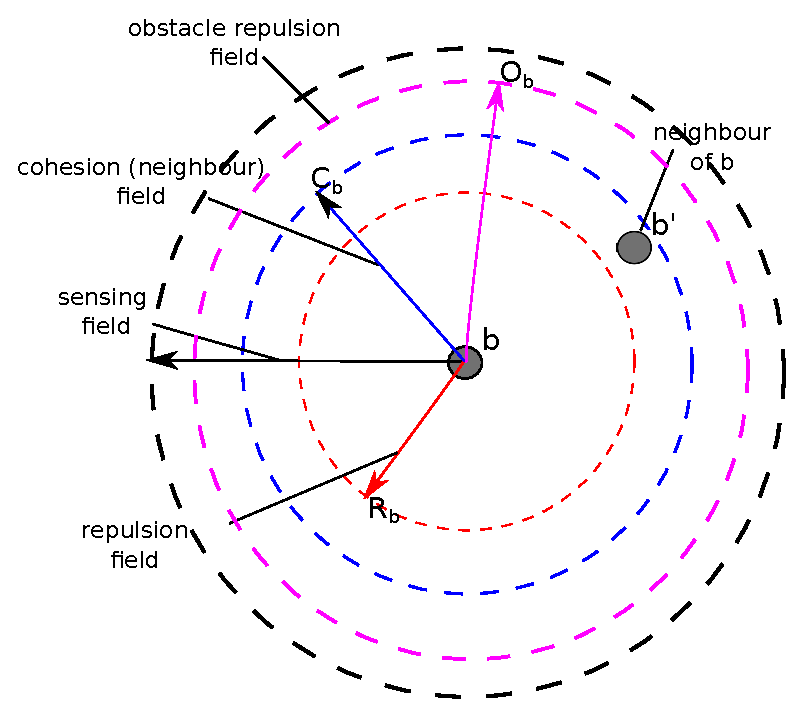
\includegraphics[width=5cm]{figures/FieldEffects}
%% \end{center}
%% \caption{Agent field effects\label{methods:FieldEffects}}
%% \end{figure}

\section{Inter-agent vector magnitude effect on internal movement}\label{Section:StabilityMagnitude}
Fig.~\ref{methods:Stability5} shows the cohesion and repulsion vector contributions to $v_c(b)$ and $v_r(b)$ due to neighbour $b'$, as given in (\ref{eq:FlyToCentre1}) and (\ref{eq:Repulsion1}). Notice that the vectors are along the line of separation $bb'$. \\

%% Equation (\ref{eq:Neighbours1}) identifies the set of agents that are neighbours of $b$.
%% 
%% \begin{equation}\label{eq:Neighbours1}
%% nbr(b) \buildrel \Delta \over = \{b' \in S | |bb'| <= C_b\}
%% \end{equation}‎

Equation~(\ref{eq:FlyToCentre1}) identifies the resultant cohesion effect of all the neighbours of $b$. Here, $nbr(b)$ defines the set of all the agents in the swarm that are a neighbour of $b$; a neighbour is any agent that fails within the cohesion field.

\begin{equation}\label{eq:FlyToCentre1}
v_{c}(b) = \frac{1}{|nbr(b)|}\left({\mathlarger{\sum_{b' \in nbr(b)}}{bb'}}\right)
\end{equation}

Equation~(\ref{eq:Repulsion1}) identifies the resultant repulsion effect of all the neighbours of $b$ where $rep(.)$ returns a set of all agents that are within the repulsion field.

\begin{equation}
\label{eq:Repulsion1}
v_{r}(b) = 
\frac{1}{|rep(b)|}
\left(
\mathlarger{\mathlarger{\sum_{b' \in rep(b)}}}
{\left( 1-\frac{|bb'|}{R_b} \right)}
{bb'}
\right)
\end{equation}

Using the cohesion and repulsion vectors generated by the relationship of $b$ to its neighbour $b'$ a resultant vector can be calculated. This vector creates an agent characteristic that can be used as a metric. Summing the vectors creates a resultant vector that affects the agent. Summing the vectors also provides an indication of the direction an agent will move based on the relationship. This is the \emph{inter-agent vector}.

Equation~(\ref{eq:InterAgentMovement1}) identifies the \emph{inter-agent vector} for agent $b$ with respect to its neighbours.

\begin{equation}\label{eq:InterAgentMovement1}
v(b) = v_{c}(b) + v_{r}(b)
\end{equation}

If a \emph{weighted} model is used then~(\ref{eq:InterAgentMovement1}) becomes~(\ref{eq:InterAgentMovement2}).

\begin{equation}\label{eq:InterAgentMovement2}
v(b) = k_cv_{c}(b) + k_rv_{r}(b)
\end{equation}

where $k_c$ and $k_r$ are weightings to change the effect of each vector as shown in Table~\ref{tab:MetricPhysics1}.

%% From here throughout sections \ref{metric:MagnitudeDynamics2} and \ref{metric:StabilityNullVector} imagine agent $b$ has just a single neighbour $b'$ and consider the effect of $b'$ on $v(b)$, the \emph{inter-agent vector} of $b$.
%% The relationship between the agents is that: \emph{the vector for $b$ with respect to $b^{'}$, and the vector for $b^{'}$ with respect to $b$ are on the same line}~(\ref{methods:Stability5}).
%% If we consider an agent ($b$) as having only one neighbour ($b'$) then using the formulae defined in chapter~\ref{chapter:methods} the vectors $v_c(b)$~(\ref{eq:FlyToCentre1}) and $v_r(b)$~(\ref{eq:Repulsion1}) are the magnitudes of the vectors that are generated by the field effects between the two agents. $k_c$ and $k_r$ are the weighting factors for the cohesion and repulsion. The resulting vectors are aligned along the same line of separation between the agents. 

\Figure[t!](topskip=0pt, botskip=0pt, midskip=0pt)[width=7cm]{figures/Stability5}
{Vectors on line of separation.\label{methods:Stability5}}

%% \begin{figure}[H]
%% \begin{center}
%% \includegraphics[width=7cm]{figures/Stability5}
%% \end{center}
%% \caption{Vectors on line of separation} \label{methods:Stability5}
%% \end{figure}

\section{Modelling movement}\label{sec:Movement1}
Each agent within a swarm calculates its \textit{movement-direction vector} based on its \textit{interaction} and \textit{destination} vectors. The \textit{movement vector}~($b_{pos}$) is calculated using the unit \textit{movement-direction vector} of (\ref{eq:InterAgentMovement2}) multiplied by the time elapsed~($t$) in the system and the speed characteristic of the agent~($s_b$).

This process is carried out for every agent in the swarm to generate the swarm's next position.

\begin{center}
\begin{equation}
\label{eq:AgentMovement}
b_{pos}=s_{b}t\big(v(b)\big)\string^ 
\end{equation}
\end{center}

The increment in the location of agent $b$ over time interval $t$ is shown in~(\ref{eq:AgentMovement}) where $s_b$ is the speed of agent~$b$. Note that \string^ is the equivalent of $\hat{v} = \frac{v}{|v|}$ the normalised vector.

\section{Swarm movement analysis\label{metric:MagnitudeDynamics2}}
The repulsion and cohesion vectors are generated for an agent through the interaction of their field effects~(Fig.~\ref{methods:FieldEffects}). There are a limited number of interactions that can occur; These are illustrated in Fig.~\ref{methods:Stability2}, \ref{methods:Stability3}, \ref{methods:Stability4} and \ref{methods:StabilityNullVector}.

Following repeated experiments in the initial deployment of a swarm it was found that using the same parameters for a swarm's environmental parameters and the cohesion and repulsion ranges that the results where always very similar. The results shown in this paper are therefore an example set typical of the results obtained. The data extracts shown in Tables \ref{tab:SampleReplusion0}, \ref{tab:SampleReplusionPositive}, \ref{tab:SampleCohesionPositive} and  \ref{tab:SampleEquilibrium} are the simulation results that are produced by the parameters listed in Table~\ref{tab:MetricPhysics1}. The simulation consists of 200 agents over a 20 second period. The cohesion of an agent pair is shown as $k_cv_c$ and the repulsion as $k_rv_r$.

\begin{table}[H]
\begin{center}
\begin{tabular}{| p{2.5cm} | c | p{3cm} |}
\hline
\bf Weight \bf Component & \bf Setting & \bf Description \\ \hline
Sample Rate & 100 & ms - Unit sampling interval\\  \hline
$k_c$ & 5 & weight adjuster for cohesion bias\\  \hline
$k_r$ & 15 & weight adjuster for repulsion  bias\\  \hline
$k_d$ & 0 & weight adjuster for directional bias 0 for static baseline 100 from directional\\  \hline
Repulsion Boundary & 70 & units\\  \hline
Neighbour Distance & 80 & units\\  \hline
Speed & 20 & units/s\\  \hline
\end{tabular}\caption{Swarm model parameters} \label{tab:MetricPhysics1}
\end{center}
\end{table}

Fig.~\ref{methods:Stability1} shows two agents within each other's cohesion fields but sufficiently distant to be outside of the repulsion fields. In this case $|k_cv_c| > 0$ and $|k_rv_r| = 0$: the result is the agent's resultant magnitude $v(b)$ causes the agent to move towards is neighbour $b'$. Likewise the neighbour's resultant magnitude $v(b')$ will cause it to move towards $b$. Table~\ref{tab:SampleReplusion0} shows the repulsion magnitude with a value of 0. The only influence on the agent pairs are cohesive vectors. 

\Figure[t!](topskip=0pt, botskip=0pt, midskip=0pt)[width=6cm]{figures/Stability1}
{Internal movement cohesion (no repulsion).\label{methods:Stability1}}

%% \begin{figure}[H]
%% \begin{center}
%% 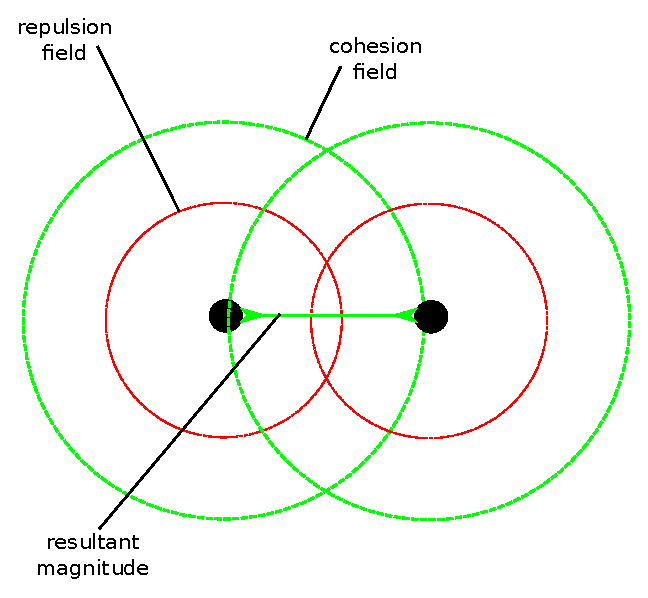
\includegraphics[width=5cm]{figures/Stability1}
%% \end{center}
%% \caption{Internal movement cohesion (no repulsion)} \label{methods:Stability1}
%% \end{figure}

\begin{table}[H]
\begin{center}
\begin{tabular}{| l | l | l | l | l | l |}
\hline
Log &	Id &	N.Id &	Distance &	{\color{green}Cohesion} &	{\color{red}Repulsion} 	\\ \hline
0 &	1 &	3 	 & 70.50359 &	{\color{green}352.51799} &	{\color{red}0} \\ \hline
0 &	1 &	100 & 71.78005 &	{\color{green}358.90027} &	{\color{red}0} \\ \hline
0 &	1 &	151 & 78.33995 &	{\color{green}391.69979} &	{\color{red}0} \\ \hline
0 &	2 &	99  &	72.04066 &	{\color{green}360.20334} &	{\color{red}0} \\ 
\hline
\end{tabular}\caption{Data extract ($|k_rv_r| = 0$)} \label{tab:SampleReplusion0}
\end{center}
\end{table}

Fig.~\ref{methods:Stability2} shows two agents close together with repulsion dominating cohesion: $|k_cv_c|~<~|k_rv_r|$. The resultant vector directs the agents away from each other. 

Table~\ref{tab:SampleReplusionPositive} shows the repulsion magnitude with a value greater than the cohesion magnitude.

\Figure[t!](topskip=0pt, botskip=0pt, midskip=0pt)[width=6cm]{figures/Stability2}
{Internal movement repulsion.\label{methods:Stability2}}

%% \begin{figure}[H]
%% \begin{center}
%% \includegraphics[width=5cm]{figures/Stability2}
%% \end{center}
%% \caption{Internal movement repulsion} \label{methods:Stability2}
%% \end{figure}

\begin{table}[H]
\begin{center}
\begin{tabular}{| l | l | l | l | l | l |}
\hline
Log &	Id &	N.Id &	Distance &	{\color{green}Cohesion} &	{\color{red}Repulsion} 	\\ \hline
0 & 1 & 2 & 28.32522 & {\color{green}141.62612} & {\color{red}1544.86014} \\ \hline
0 & 1 & 6 & 41.48517 & {\color{green}207.42586} & {\color{red}721.71736} \\ \hline
0 & 1 & 7 & 35.26412 & {\color{green}176.32064} & {\color{red}1034.27101} \\ \hline
0 & 1 & 8 & 43.54503 & {\color{green}217.72518} & {\color{red}637.90759} \\
\hline
\end{tabular}\caption{Data extract ($|k_cv_c| < |k_rv_r|$)} \label{tab:SampleReplusionPositive}
\end{center}
\end{table}

Fig.~\ref{methods:Stability3} shows two agents close together but with cohesion vector magnitudes greater than the repulsion magnitudes $|k_cv_c|~>~|k_rv_r|$. The resultant vector draws the agents together. The magnitude of the resultant cohesion vector reduces due to the cancelling effect of the repulsion vector. Table~\ref{tab:SampleCohesionPositive} shows a data extract with the cohesion magnitude greater than repulsion.

\Figure[t!](topskip=0pt, botskip=0pt, midskip=0pt)[width=6cm]{figures/Stability3}
{Internal movement cohesion and repulsion.\label{methods:Stability3}}

%% \begin{figure}[H]
%% \begin{center}
%% 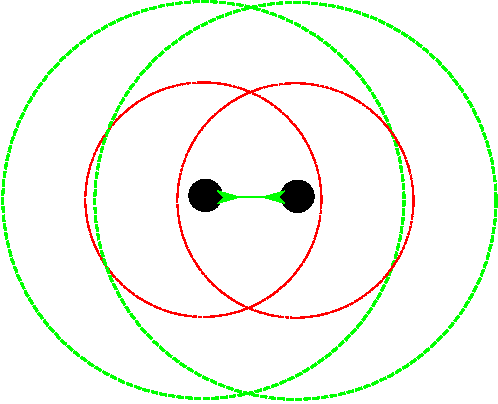
\includegraphics[width=5cm]{figures/Stability3}
%% \end{center}
%% \caption{Internal movement cohesion and repulsion} \label{methods:Stability3}
%% \end{figure}

\begin{table}[H]
\begin{center}
\begin{tabular}{| l | l | l | l | l | l |}
\hline
Log &	Id &	N.Id &	Distance &	{\color{green}Cohesion} & {\color{red}Repulsion} 	\\ \hline
0 & 1 & 5 &	64.17214 &	{\color{green}320.86072} &	{\color{red}95.35676} \\ \hline
0 & 1 & 9 &	63.88049 &	{\color{green}319.40248} &	{\color{red}100.58590} \\ \hline
0 & 1 & 95 & 65.61522 &	{\color{green}328.07613} &	{\color{red}70.16681} \\ \hline
0 & 1 & 152 & 63.10700 & {\color{green}315.5350} & {\color{red}114.68844} \\ 
\hline
\end{tabular}\caption{Data extract ($|k_cv_c| > |k_rv_r|$)} \label{tab:SampleCohesionPositive}
\end{center}
\end{table}

Fig.~\ref{methods:Stability4} shows two agents close together with $|k_cv_c|~=~|k_rv_r|$ the resultant vector is a \emph{null vector} and the agents have no overall influence upon each other due to the magnitude of the resultant vector being zero. Table~\ref{tab:SampleEquilibrium} is an extract of data from the simulator. The data shows near equilibrium but due to the dynamic nature of a swarm system no agents meet the condition fully. 

\Figure[t!](topskip=0pt, botskip=0pt, midskip=0pt)[width=6cm]{figures/Stability4}
{Internal movement equilibrium.\label{methods:Stability4}}

%% \begin{figure}[H]
%% \begin{center}
%% 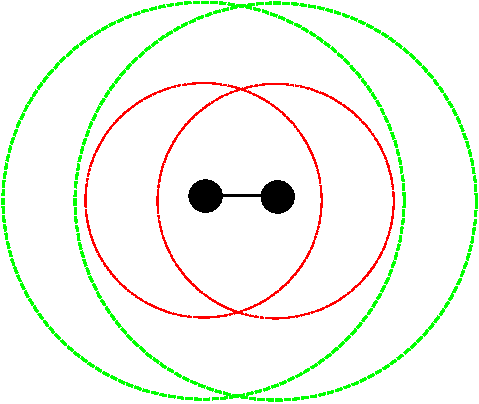
\includegraphics[width=5cm]{figures/Stability4}
%% \end{center}
%% \caption{Internal movement equilibrium} \label{methods:Stability4}
%% \end{figure}

\begin{table}[H]
\begin{center}
\begin{tabular}{| l | l | l | l | l | l |}
\hline
Log &	Id &	N.Id &	Distance &	{\color{green}Cohesion} &	{\color{red}Repulsion} 	\\ \hline
7 & 76 &	91 & 55.39031 & {\color{green}276.95156} & {\color{red}276.94684} \\ \hline
24 & 75 & 6 & 55.39032 & {\color{green}276.95160} & {\color{red}276.94661} \\ \hline
32 & 72 & 38 &	55.39002 & {\color{green}276.95013} & {\color{red}276.95370} \\ \hline
35 & 63 & 64 & 55.39022 &	{\color{green}276.95113} &	{\color{red}276.94887} \\
\hline
\end{tabular}\caption{Data extract ($|k_cv_c| \approx |k_rv_r|$)} \label{tab:SampleEquilibrium}
\end{center}
\end{table}

\section{Internal movement and the null vector}\label{section:StabilityNullVector}
When the two vectors (cohesion and repulsion) have magnitudes that are equal and opposite they produce a null vector, indicating that two agents are optimally spaced for a given set of conditions. Although the agents are at an optimum position when resultants are zero it does not mean the swarm is optimally distributed. If a swarm is in a confined space it is possible for an optimum position to be created where the vector magnitude is affected by a compression effect. This phenomenon is used in the identification of the emergent behaviour of \emph{area flooding}.  

If we consider the equilibrium state (Fig.~\ref{methods:Stability4}) the resultant $v(b)=(0,0)$. A null vector cannot be normalised to produce a directional vector ($\hat{v} = \frac{v}{|v|}$ if $v\neq0$; $0$ if $v=0$) The effect is that the agent will remain stationary. If all agent pairs are in this condition the swarm will stop moving~(Fig.~\ref{methods:StabilityNullVector}).

\Figure[t!](topskip=0pt, botskip=0pt, midskip=0pt)[width=5cm]{figures/StabilityNullVector}
{Equilibrium with null vectors.\label{methods:StabilityNullVector}}

%% \begin{figure}[H]
%% \begin{center}
%% \includegraphics[width=5cm]{figures/StabilityNullVector}
%% \end{center}
%% \caption{Equilibrium with null vectors} \label{methods:StabilityNullVector}
%% \end{figure}

Due to the movement of agents being based only on neighbour interactions this situation is very rare. The residual motion that persists in a swarm is the background `noise' or `jitter' that an algorithm creates.

If a swarm is goal-based, the addition of a \emph{directional vector} will prevent all agents simultaneously producing null vectors as shown in~(Fig.~\ref{concave:VoidPerimeter2}, Equation~(\ref{eq:InterAgentMovementDirectional1})). Here, $k_dv_{d}(b)$ is the calculated directional vector to be applied to an agent.

\begin{equation}\label{eq:InterAgentMovementDirectional1}
v(b) = k_cv_{c}(b) + k_rv_{r}(b) + k_dv_{d}(b)
\end{equation}

\Figure[t!](topskip=0pt, botskip=0pt, midskip=0pt)[width=5.5cm]{figures/StabilityNullVector3}
{(t).\label{concave:VoidPerimeter1}}

%% \begin{figure}[H]
%% \begin{center}
%% 	 \includegraphics[width=5.5cm]{figures/StabilityNullVector3}
%% \end{center}
%% \label{concave:VoidPerimeter1}
%% \caption{(t)}
%% \end{figure}

\Figure[t!](topskip=0pt, botskip=0pt, midskip=0pt)[width=6cm]{figures/StabilityNullVector2}
{(t + 1).\label{concave:VoidPerimeter2}}

%% \begin{figure}[H]
%% \begin{center}
%% 	 \includegraphics[width=6cm]{figures/StabilityNullVector2}
%% \end{center}
%% \caption{(t + 1)}
%% \label{concave:VoidPerimeter2}
%% \end{figure}

\section{Residual internal movement (Jitter)}\label{metric:Jitter}
Due to the dynamic nature of a swarm, maintaining optimum internal movement as in~Figure \ref{methods:StabilityNullVector} is highly unlikely. The agent pairs may fluctuate between the 4 states~(Fig.~\ref{methods:Stability1}, \ref{methods:Stability2}, \ref{methods:Stability3} and \ref{methods:Stability4}); These transitions are \emph{jitter}. The degree to which this variation occurs can be measured using either the change in distance between the agents, or the change in the magnitude $P(b)$~(\ref{eq:CohesionRepulsion}) between the agents. Jitter arises as motion to maintain the structure of a swarm. A swarm coordination algorithm that reduces jitter is generally desirable. 

\section{Distance metric\label{section:DistanceDynamics}}
The distance metric considers a swarm in terms of how the agents are physically distributed: i.e. only the inter-agent distances and their standard deviation are considered. The standard deviation indicates the extent to which the swarm is out of balance and will move to re-balance itself. If the standard deviation is zero then all the agents are evenly spaced. 

%The distance metric does not take into consideration the vector magnitudes between the agents as discussed above. The metric therefore is unable to identify the potential state of the swarm in terms of its cohesive or repulsive state.

Navarro and Fernando describe a \emph{mean distance error} metric that is based on the variations in distances between inter-agent spaces~\cite{NIM:09}. This is the same as the standard deviation of the distance based internal movement metric. 


%% \section{Distance metric internal movement}
%% The distance based internal movement is measured by identifying the mean length of the vectors between an agent and its neighbours. As with the \emph{agent resultant magnitude} a coordination algorithm produces `jitter' which is the variations from the mean. In the case of the distance based metric the jitter is identified by the changes in the distances rather than the changes in vector magnitude (\emph{agent resultant magnitude}). The distance metric is the mean and the standard deviation `jitter' of the inter-agent distances.

\section{Calculating distance internal movement}
Equation~(\ref{eq:SwarmStabilityDistance1}) computes the mean distance of an agent to its neighbours $nbr(b)$. 
%% The relative position vector generated for an agent $b$ to its neighbour $b'$, $bb'$, is shown in~(\ref{eq:FlyToCentre1}). The magnitude of that vector gives the distance between two agents. For an individual agent the average magnitude $\mu_d(b)$ is calculated as \ref{eq:SwarmStabilityDistance1} where $b$ is the agent and $|nbr(b)|$ is the number of neighbours.

\begin{equation}
\label{eq:SwarmStabilityDistance1}
\mu_d(b) = \frac{1}{\mathlarger{|nbr(b)|}}\left({\mathlarger{\sum_{b' \in nbr(b)}}|bb'|}\right)
\end{equation}

The mean distance for a swarm is calculated by~(\ref{eq:SwarmStabilityDistance2}). All the inter-agent distances are included for the swarm ($S$). 

%% $\sum_{b \in S}|nbr(b)|$ calculates how many inter-agent relationships exist in the swarm and $\sum_{b' \in nbr(b)}|bb'|$ calculates the total distance between each agent and its neighbours. $\sum_{b \in S}$ iterates over all the agents in the swarm~($S$).

\begin{equation}
\label{eq:SwarmStabilityDistance2}
\mu_d(S) = \frac{\mathlarger{\sum_{b \in S}}~\mathlarger{\sum_{b' \in nbr(b)}}|bb'|}{\mathlarger{\sum_{b \in S}|nbr(b)|}}
\end{equation}

%\section{Standard deviation in distance metric}\label{Section:VarianceInDistance}
The mean distance provides a indication of the large scale structure of the swarm. However it is not sufficient to give an indication of the internal distribution of the agents. The standard deviation clarifies the distribution within the swarm as shown in~(\ref{eq:SwarmStabilityDistance3}). 

%% $(|bb'| - \mu(S))^2$ is the square of the difference in a distance to the mean and $\sum_{b \in S}~\sum_{b' \in nbr(b)}$ calculates the number of inter-agent interactions.

\begin{equation}
\label{eq:SwarmStabilityDistance3}
\sigma_d(S) = \sqrt{\frac{\mathlarger{\sum_{b \in S}}~\mathlarger{\sum_{b' \in nbr(b)}}\Big(|bb'| - \mu_d(S)\Big)^2}{\mathlarger{\sum_{b \in S}|nbr(b)|}}}
\end{equation}

The distance-based metric for the internal distribution of the agents is the pair consisting of $\mu_d(S)$, $\sigma_d(S)$. This can be written informally as:

\begin{equation}
\label{eq:SwarmDistanceMetric}
\psi_d(S) = \mu_d(S)\pm \sigma_d(S)
\end{equation}

\Figure[t!](topskip=0pt, botskip=0pt, midskip=0pt)[width=14cm]{figures/BaselineDistance1}
{Baseline internal movement - distance.\label{coord:BaselineDistance1}}

%% \begin{figure}[H]
%% \begin{center}
%% 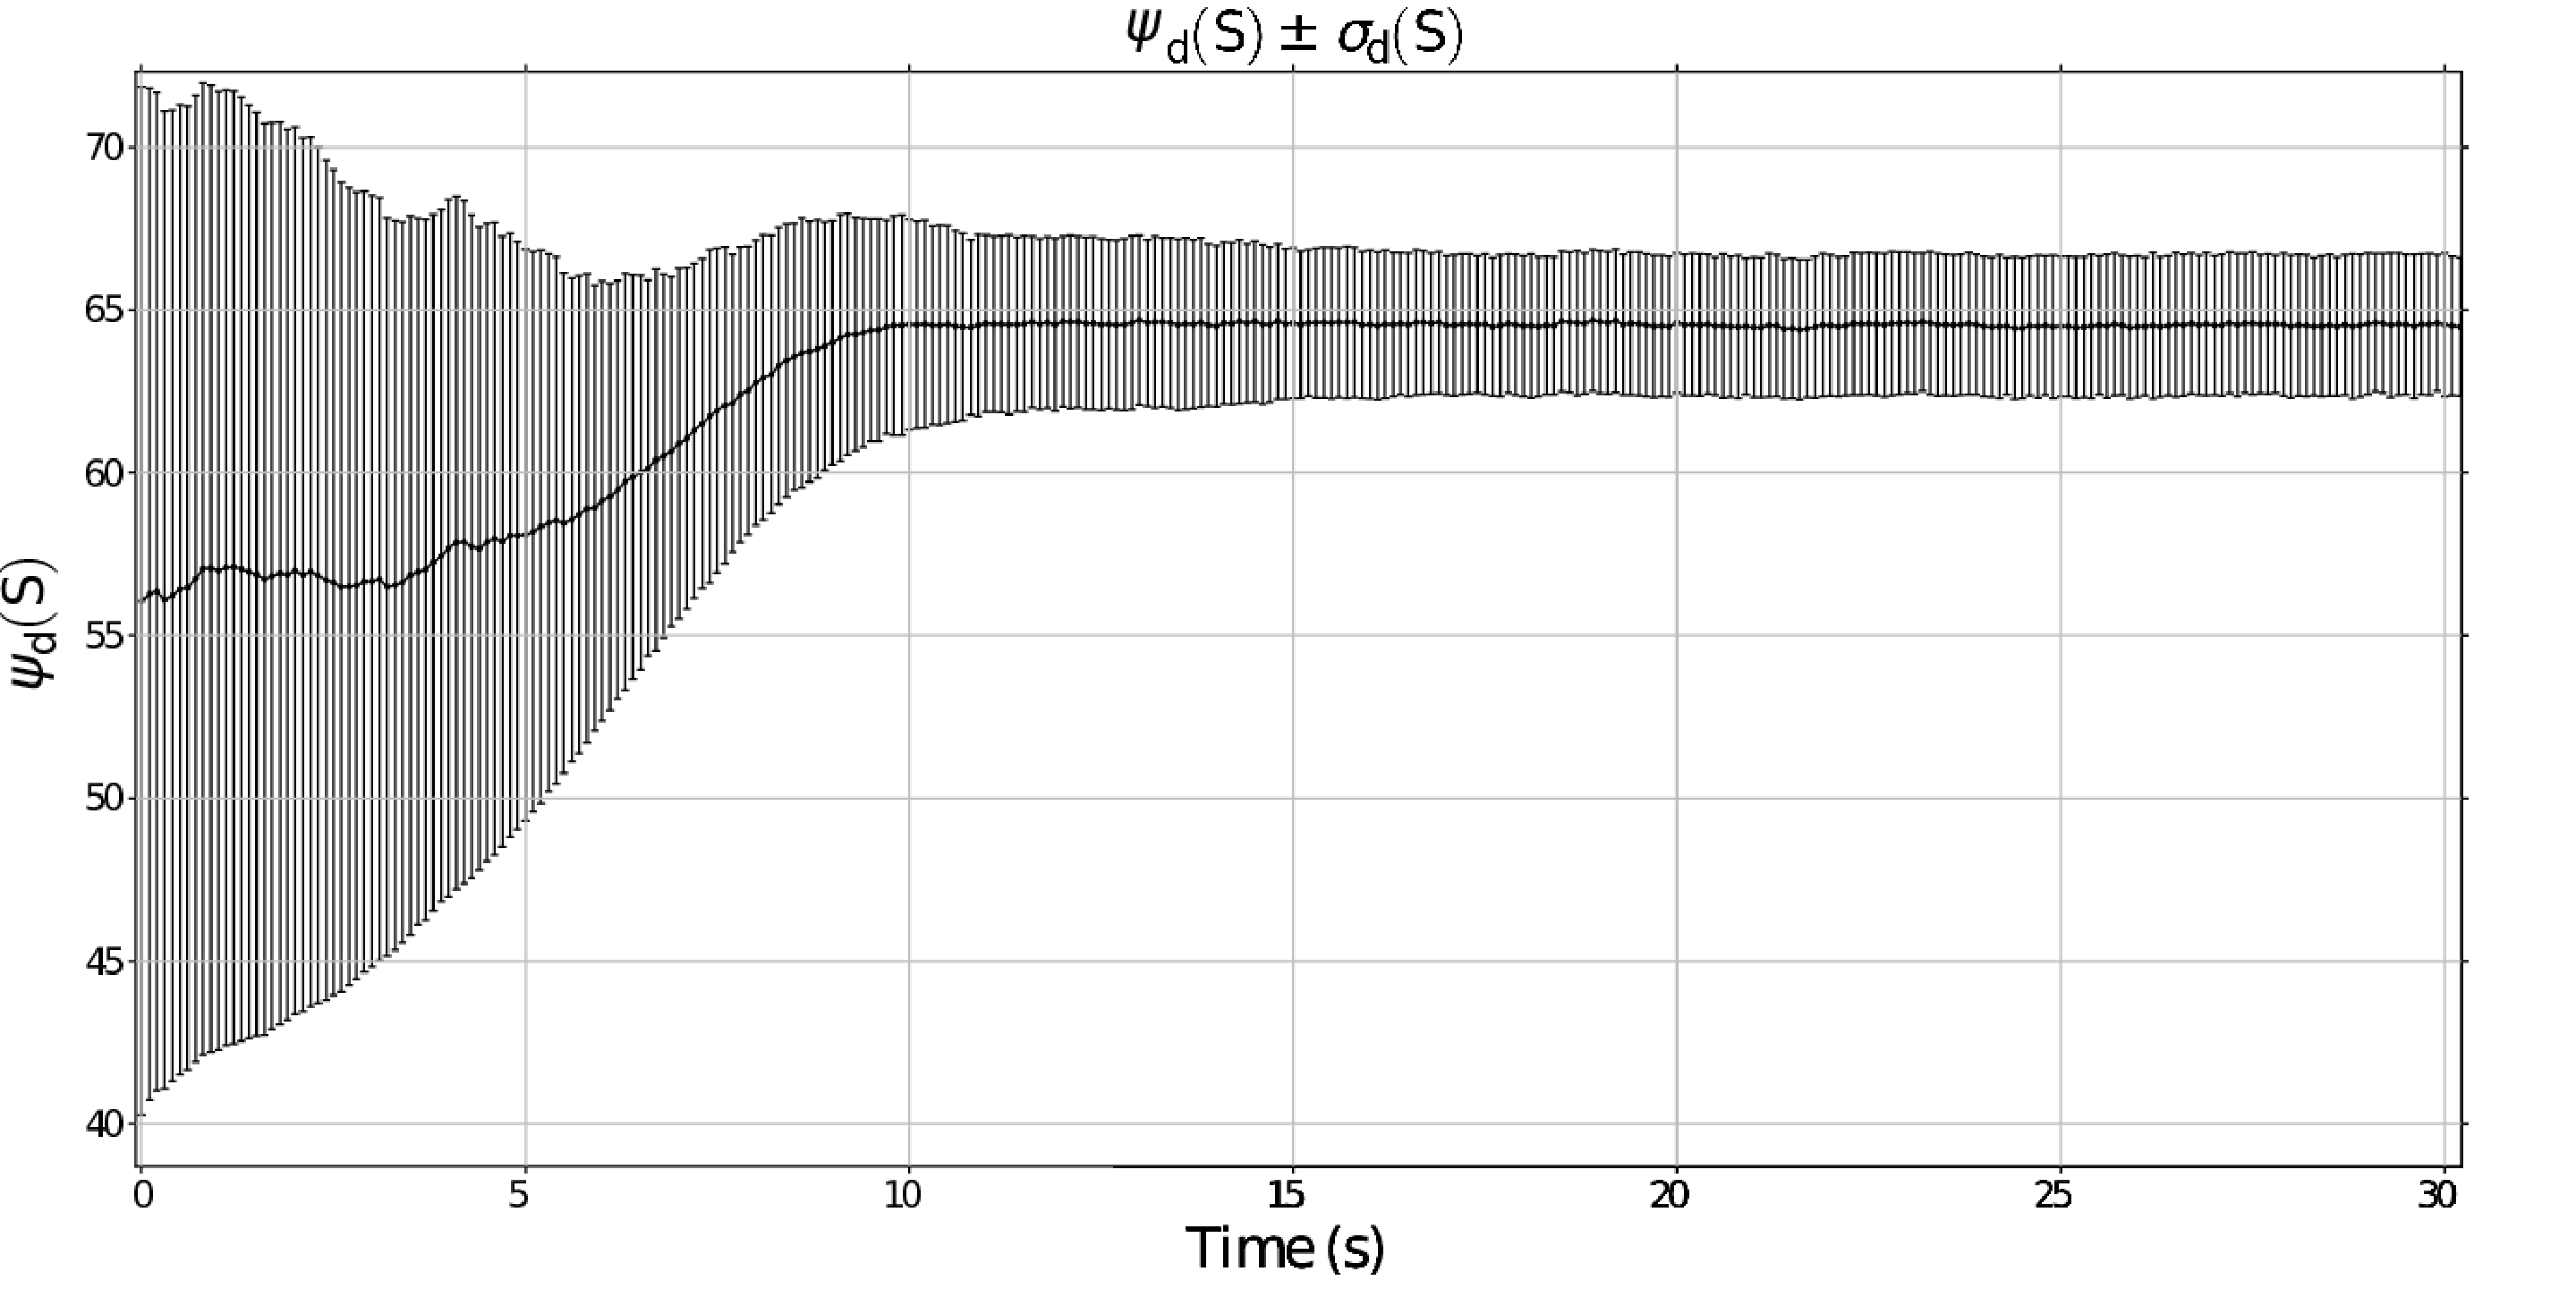
\includegraphics[width=9cm]{figures/BaselineDistance1}
%% \end{center}
%% \caption{Baseline internal movement - distance\label{coord:BaselineDistance1}}
%% \end{figure}

\section{Cohesion/repulsion metric\label{section:MagnitudeDynamics}}
% An agent's \emph{resultant magnitude} is identified by Gazi and Passino~\cite{GP:11} and Barnes et al~\cite{BFV:07} as a `resultant characteristic' of a swarm. The sum of the cohesion and repulsion vectors between an agent $b$ and a neighbour $b'$ produce a resultant vector.

% The cohesion/repulsion internal movement (\emph{cohesion/repulsion metric}) is measured by identifying the balance between the cohesion and repulsion vectors between agents as shown in~(\ref{eq:CohesionRepulsion}). This is derived from the \emph{inter-agent cohesion/repulsion vector} as shown in~(\ref{eq:InterAgentMovementDirectional1}). `Jitter' in the case of the agent resultant \emph{cohesion/repulsion metric} is measured as the deviation created by the inter-agent relationships. The identification of this deviation produces the clarifying component of the agent \emph{cohesion/repulsion metric}.
% %% The magnitude based metric identifies the resultant internal magnitude (vector magnitude) through the cohesive and repulsive magnitudes that exist between each agent pair in a swarm. 
% An agent's resultant vector magnitude is used as a scalar value to give an overall `size' to the agent relationship. The resultant scalar value is then modified based upon the `size' of the two relationship magnitudes.

% This paper will refer to the scalar resultant magnitude as the \emph{`cohesion/repulsion metric'} of the relationship. The `state' of a swarm is therefore the effect the environmental constraints and algorithms have upon the agent resultant magnitude. The agent's \emph{`cohesion/repulsion metric'} can be considered part of the `quality' measure for a swarm's performance.

% The resultant \emph{cohesion/repulsion metric}, which is a scalar, is generated by comparing the length of the cohesion and repulsion vector magnitudes. If the cohesion magnitude is larger than the repulsion vector magnitude the resultant length is considered to be positive. If the repulsion vector magnitude is larger than the cohesion vector magnitude the resultant length is considered to be negative. 

% The \emph{`cohesion/repulsion metric'} is therefore the scalar value of the \emph{`agent resultant magnitude'} which is altered based upon the difference between the repulsion and cohesion magnitudes~(\ref{eq:CohesionRepulsion}).
This paper defines the cohesion/repulsion metric scalar for an agent as the length of $v(b)$  as defined (\ref{eq:InterAgentMovement2}): that is, the weighted effects of cohesion and repulsion by neighbours of the agent. This number carries a negative sign if repulsion dominatesand a positive sign if cohesion dominates and a positive sign if cohesion donates. This is summarised by~(\ref{eq:CohesionRepulsion}).

If an agent's {cohesion/repulsion metric} is negative the swarm's bias is to expand as the repulsion is greater than cohesion. This is seen in the disorganised stage of a swarm~(Fig.~\ref{coord:BaselineMagnitude1}). The disorganised stage is the initial random deployment of the agents. If the agent \emph{agent resultant magnitude} is positive then the swarm is exhibiting a tendency to contract and this indicates the swarm is a cohesive entity. This could also be described as the swarm being `sticky' as the agents bias is to `pull' towards each other.

The \emph{cohesion/repulsion metric} on its own does not give a complete measure of a swarm's internal state. There needs to be a qualifying component to the metric that identifies the degree of deviation in the resultant magnitude, this is the \emph{jitter}. The smaller the deviation the more uniform the structure of the swarm. These two components identify the degree to which a swarm has progressed towards a stable state.
 
The \emph{cohesion/repulsion metric} provides a view of the swarm's state through the balance between the repulsive and the cohesive vectors that are being applied to each agent. The deviation component identifies the degree to which the swarm has stabilised. The ideal status for inter-agent interactions would be for the agents to have a (\emph{cohesion/repulsion metric}) of zero or above. This would indicate that the agents are distributed such that they are at their distribution limit (outer most range of the cohesion field) or at a level that causes the agents to `pull' together. The ideal degree of deviation is zero as this indicates an even distribution of agents. These two aspects of a swarm's features are not considered by Gazi and Passino~\cite{GP:11} or Barnes et al~\cite{BFV:07} as a means of quantifying the structure of a swarm in terms of stability.

\section{Cohesion/repulsion internal movement model}\label{Section:StabilityModel}
Section~\ref{Section:StabilityMagnitude}~discussed calculation of resultant cohesion~(\ref{eq:FlyToCentre1}) and resultant repulsion~(\ref{eq:Repulsion1}) vectors for each agent deriving a combined \emph{cohesion/repulsion vector} using~(\ref{eq:InterAgentMovement2}). 

%% This value represents the overall `potential' of an agent. This vector when normalised produces a component of the \emph{movement-destination vector} for a swarm. If the total cohesion/repulsion vector is zero (null vector) then the agent will not move. $M(b)$ is the total \emph{cohesion/repulsion vector} for agent $b$ defined by:
%% 
%% \begin{equation}
%% \label{eq:BotStabilityT}
%% M(b) = k_cv_c(b) + k_rv_r(b)
%% \end{equation}

Now, we define for each agent $b$ a \emph{cohesion/repulsion scalar}, $P(b)$, to measure the influence of the neighbours of $b$ on $b$ as cohesive (positive) or repulsive (negative); this is~(\ref{eq:CohesionRepulsion}).

\begin{equation}
\label{eq:CohesionRepulsion}
P(b) = \left\{\begin{array}{lll}
               |v(b)|& \mathrm{if} & |k_cv_c(b)| > |k_r v_r(b)|\\
              -|v(b)|& \mathrm{otherwise}
              \end{array}\right.
\end{equation}

Although it is possible for $v(b)$ to be null there could still be variation in the constituent components. The variation calculation (standard deviation) is shown below. 

%% Equation~\ref{eq:SwarmStabilityMetricT} is the mean of the cohesion/repulsion scalar for an agent.
%% 
%% \begin{equation}
%% \label{eq:SwarmStabilityMetricT}
%% \mu_p(b) = \frac{P(b)}{|nbr(b)|}
%% \end{equation}

%% \ref{eq:SwarmStabilityMetricT} should be considered as being applied at discrete points in time within a simulation. The formulae could also be shown based on time $t$ (\ref{eq:SwarmStabilityMetricT2}) where $b_t$ is an agent at a specific time interval. All formulae for agent resultant magnitude in this thesis will be considered as being applied at a point in time and will therefore be shown without a $t$ subscript.
%% 
%% \begin{equation}
%% \label{eq:SwarmStabilityMetricT2}
%% \mu_p(b_{t}) = \frac{P(b_{t})}{|nbr(b_{t})|}
%% \end{equation}

The mean cohesion/repulsion scalar for the swarm is now given by~(\ref{eq:SwarmStabilityMetricT3}).  

\begin{equation}
\label{eq:SwarmStabilityMetricT3}
\mu_p(S) = \frac{\mathlarger{\sum_{b \in S} P(b)}}{\mathlarger{\sum_{b \in S}}|nbr(b)| + \mathlarger{\sum_{b \in S}}|rep(b)|}
\end{equation}

%% \section{Standard deviation in agent cohesion/repulsion metric}\label{Section:VarianceInPotential}
%% To improve the metric clarification in terms of the deviation from the \emph{cohesion/repulsion metric} norm is calculated. The standard deviation of the entire swarm  is shown in Equation \ref{eq:SwarmStabilityMetricT}.

The standard deviation associated with this mean is calculated as~(\ref{eq:SwarmStabilityQuotientT}).
%%  where $\sigma_p(S)$ is the standard deviation and $\mu_p(S)$ is the mean at the same point in time. 

\begin{equation}
\label{eq:SwarmStabilityQuotientT}
\sigma_p(S) = \sqrt{\frac{\mathlarger{\sum_{b \in S}}\Big(P(b)-\mu_p(S)\Big)^2}{\mathlarger{\sum_{b \in S}}|nbr(b)| + \mathlarger{\sum_{b \in S}}|rep(b)|}}
\end{equation}

The metric for the internal movement is this pair of numbers, the mean and standard deviation of the swarm's internal \emph{cohesion/repulsion}. The pair $\mu_p(S)$, $\sigma_p(S)$ may be written informally as: 

\begin{equation}
\label{eq:SwarmPotentialMagnitude}
\psi_p(S) = \mu_p(S)\pm \sigma_p(S)
\end{equation}

Figure~\ref{coord:BaselineMagnitude1} shows the evolution of the metric in time.

\Figure[t!](topskip=0pt, botskip=0pt, midskip=0pt)[width=14cm]{figures/BaselineMagnitude1}
{Baseline internal movement - cohesion/repulsion.\label{coord:BaselineMagnitude1}}

%% \begin{figure}[H]
%% \begin{center}
%% 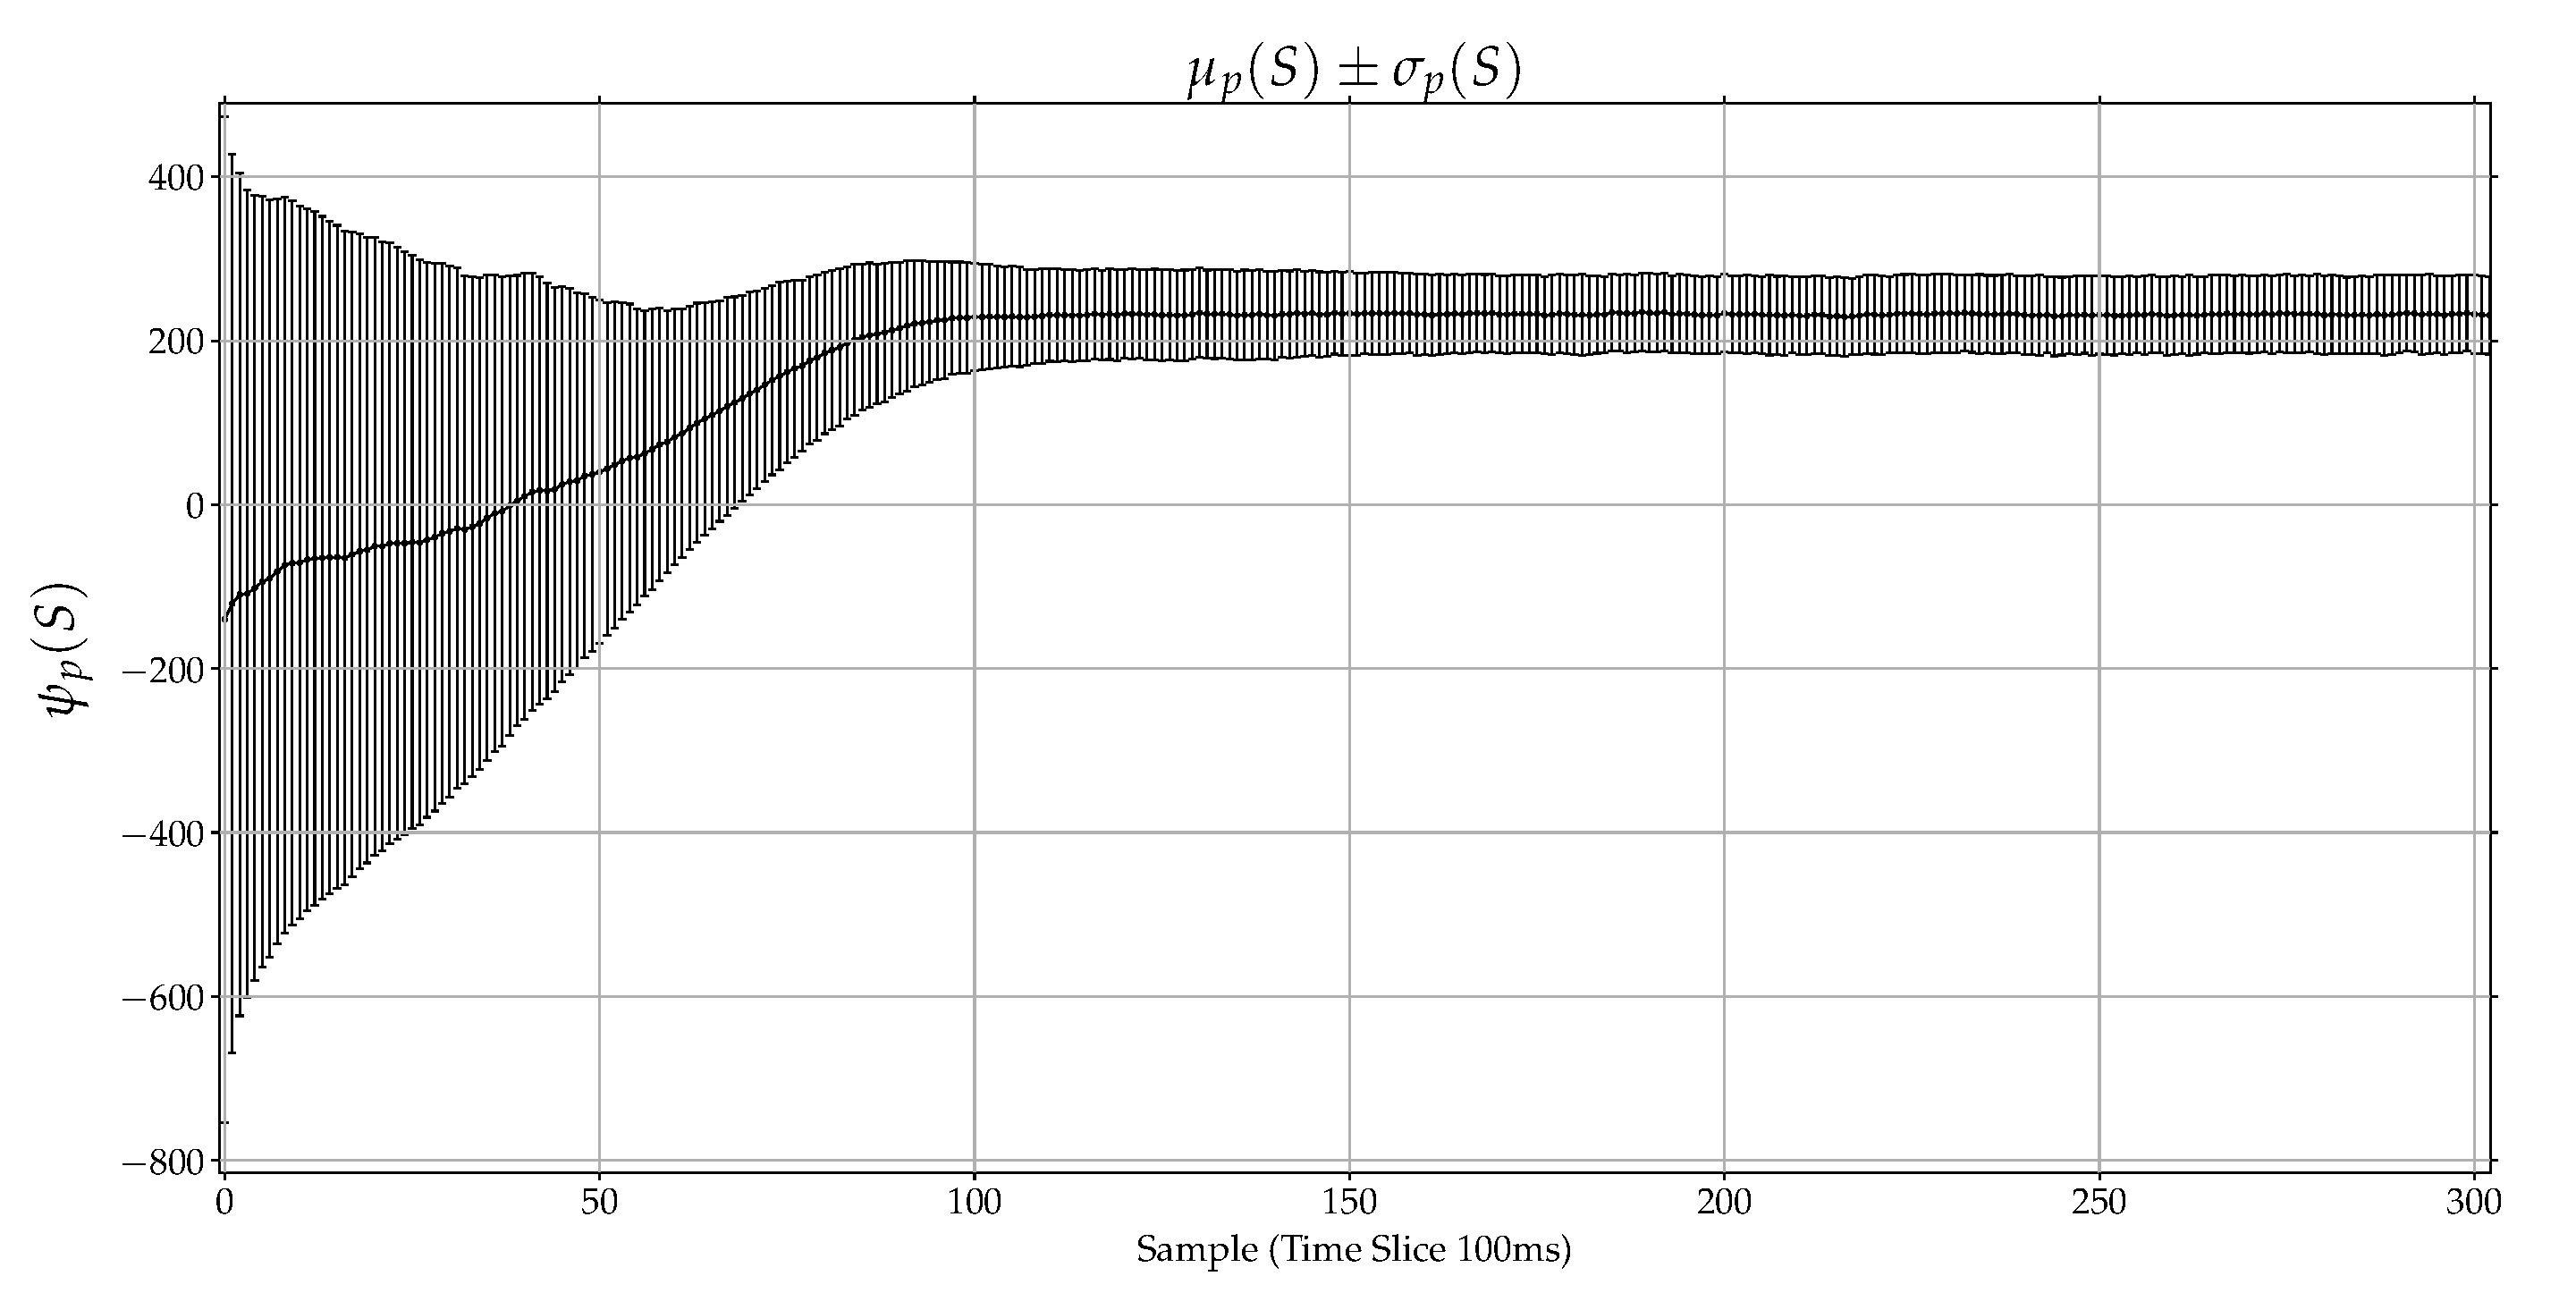
\includegraphics[width=9cm]{figures/BaselineMagnitude1}
%% \end{center}
%% \caption{Baseline internal movement - magnitude\label{coord:BaselineMagnitude1}}
%% \end{figure}

\section{Application: Area filling}\label{metric:ApplicationFloodFilling}

Area filling is a technique used to fill an enclosed area with agents such that they are distributed as `effectively' as possible throughout an area. 

Filling an area can be applied to tasks that require an unknown environment to be analysed or surveyed. Consider a disaster area following a landslide or a building collapse following an earthquake; the movement in the land and buildings will produce areas that are unmapped. The unmapped areas may require investigation to locate people, or resources, or to create some form of sensor network to analyse the conditions within the area, such as creating a heat map or identifying the location of toxic gases. 

The concept of using a swarm to provide coverage over unknown areas is a current area of research. Alvissalim et al. (2012) discuss the application of commercially available drones to provide a communication infrastructure across an unmapped disaster area~\cite{AZHMJJM:12}. Scheutz and Bauer (2006) use both cohesion and repulsion as a mechanism to create coverage of an area that requires protection in an adversarial environment~\cite{SB:06}.

The concept behind the area filling is to increase both the repulsion and cohesion fields over a period of time. This increase in the field effects makes the agents increase the distance between each other, expanding the swarm as a whole. The expansion increases until, due to boundary compression, the swarm is unable to expand further. In an extreme case the expansion will result in a set of field effects that create a mesh based swarm structure rather than the desired hexagonal structure that the field effects should create. Identifying the \textit{cohesion/repulsion metric} falling below zero indicates area saturation has occurred.

To test this hypothesis a swarm is modelled in the simulator. The model consists of an obstacle-based enclosed space and a swarm consisting of 60 agents. The experiments parameters for the simulation are shown in~Table~\ref{tab:FillParameters1}

\begin{table}[H]
\begin{center}
\begin{tabular}{| p{1.8cm} | p{1.5cm} | p{4.0cm} |}
\hline
\bf Parameter & \bf Value  & \bf Description \\ \hline
$k_c$         & 5          & weight adjuster for cohesion bias\\ \hline
$k_r$         & 60         & weight adjuster for repulsion bias\\ \hline
Sample rate   & 100ms      & proximity sensor rate\\ \hline
Speed         & 20 units/s & agent speed\\ \hline
\end{tabular}\caption{Swarm parameters} \label{tab:FillParameters1}
\end{center}
\end{table}

The field effects are incremented in turn, cohesion range followed by repulsion range. After each repulsion field change the swarm is allowed to redistribute itself and stabilise. Table~\ref{tab:FillSequence} shows the field effect settings that are used for the simulation. The field effects are selected so as to ensure the swarm parameters have the potential to create a hexagonal swarm. Figure \ref{emerge:FLOOD0} shows the initial swarm deployment.

\Figure[t!](topskip=0pt, botskip=0pt, midskip=0pt)[width=8cm]{figures/FLOOD0}
{Flood fill Start.\label{emerge:FLOOD0}}

Fig.~\ref{emerge:FLOOD1} shows the point a which data logging starts. The swarm at this stage has expanded into the space but is not filling it. This presents itself as a positive cohesion/repulsion metric value which indicates the swarm is cohesive and the agents are still ``pulling" together. Fig.~\ref{emerge:FLOOD6} shows the final swarm distribution for the simulation, at this point the cohesion/repulsion metric has fell below zero indicating the swarm is trying to expand. 

\Figure[t!](topskip=0pt, botskip=0pt, midskip=0pt)[width=8cm]{figures/FLOOD1}
{Data Capture Start.\label{emerge:FLOOD1}}

\Figure[t!](topskip=0pt, botskip=0pt, midskip=0pt)[width=8cm]{figures/FLOOD6}
{Flood fill End.\label{emerge:FLOOD6}}

\begin{table}[H]
\begin{center}
\begin{tabular}{| p{1.8cm} | p{0.3cm} | p{0.3cm} | p{0.3cm} | p{0.3cm} | p{0.3cm} | p{0.3cm} | p{0.3cm} | p{0.7cm} |}
\hline
\bf Weight \bf component & \bf 1 & \bf 2 & \bf 3 & \bf 4 & \bf 5 & \bf 6 & \bf 7 & \\ \hline
Repulsion Boundary & 50 & -  & 60 & -  & 70 & -  & 80 & units\\  \hline
Neighbour Distance & 60 & 70 & -  & 80 & -  & 90 & -  & units\\  \hline
\end{tabular}\caption{Field effect expansion sequence} \label{tab:FillSequence}
\end{center}
\end{table}

Fig.~\ref{emerge:FIELDFILL-MAG} shows the cohesion/repulsion metric for the swarm for the entire simulation. Between 100 seconds and 105 seconds there is a significant change in the magnitude where the value becomes negative. This indicates there is a compression effect on the swarm which indicates the area is filled.

\Figure[t!](topskip=0pt, botskip=0pt, midskip=0pt)[width=13cm]{figures/FIELDFILL-MAG}
{Cohesion/Repulsion metric 0-120 seconds.\label{emerge:FIELDFILL-MAG}}

% \begin{figure}[H]
% \begin{center}
% 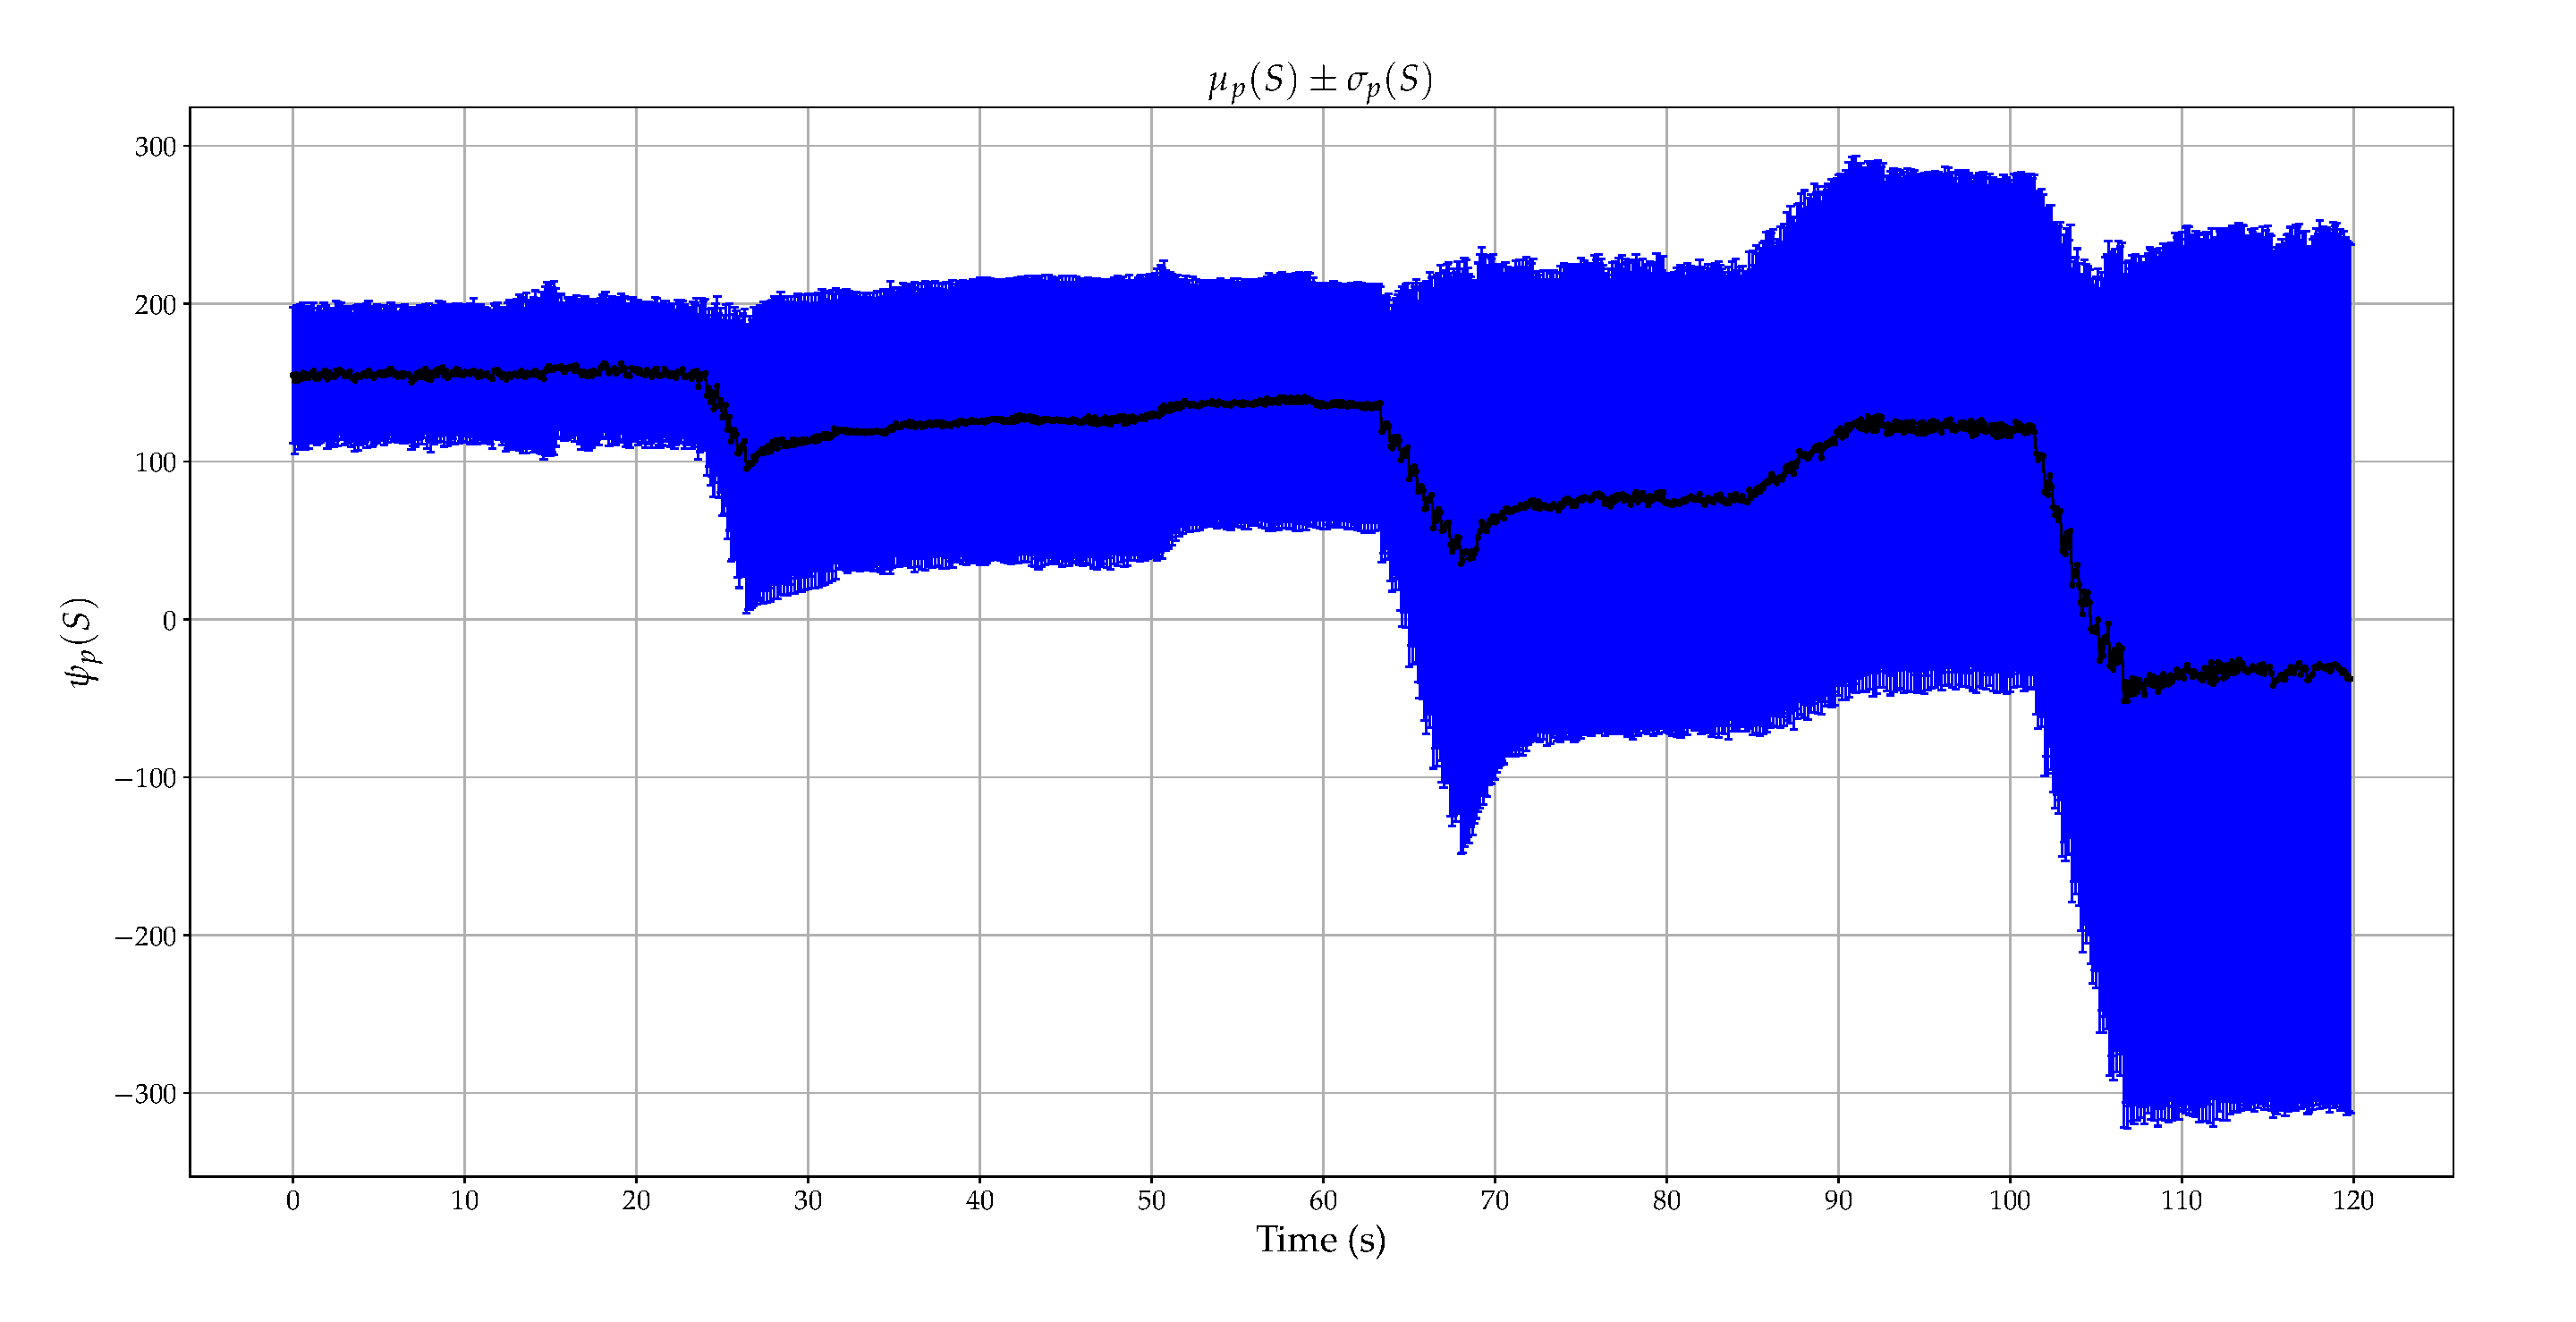
\includegraphics[width=12cm]{figures/FIELDFILL-MAG}
% \end{center}
% \caption{Magnitude metric 0-120 seconds\label{emerge:FIELDFILL-MAG}}
% \end{figure}

Fig.~\ref{emerge:FIELDFILL-DIST}~shows the distance metric for the same simulation. The initial deployment is shown at 0 seconds followed by incremental changes in the distances and variance of the distances as each increment is made in the field effects. The simulation terminates after 120 seconds. There is no feature of this graph which indicates that the area is filled. The cohesion/repulsion metric clearly tells us more. 

\Figure[t!](topskip=0pt, botskip=0pt, midskip=0pt)[width=13cm]{figures/FIELDFILL-DIST}
{Distance metric 0-120 seconds.\label{emerge:FIELDFILL-DIST}}

% \begin{figure}[H]
% \begin{center}
% 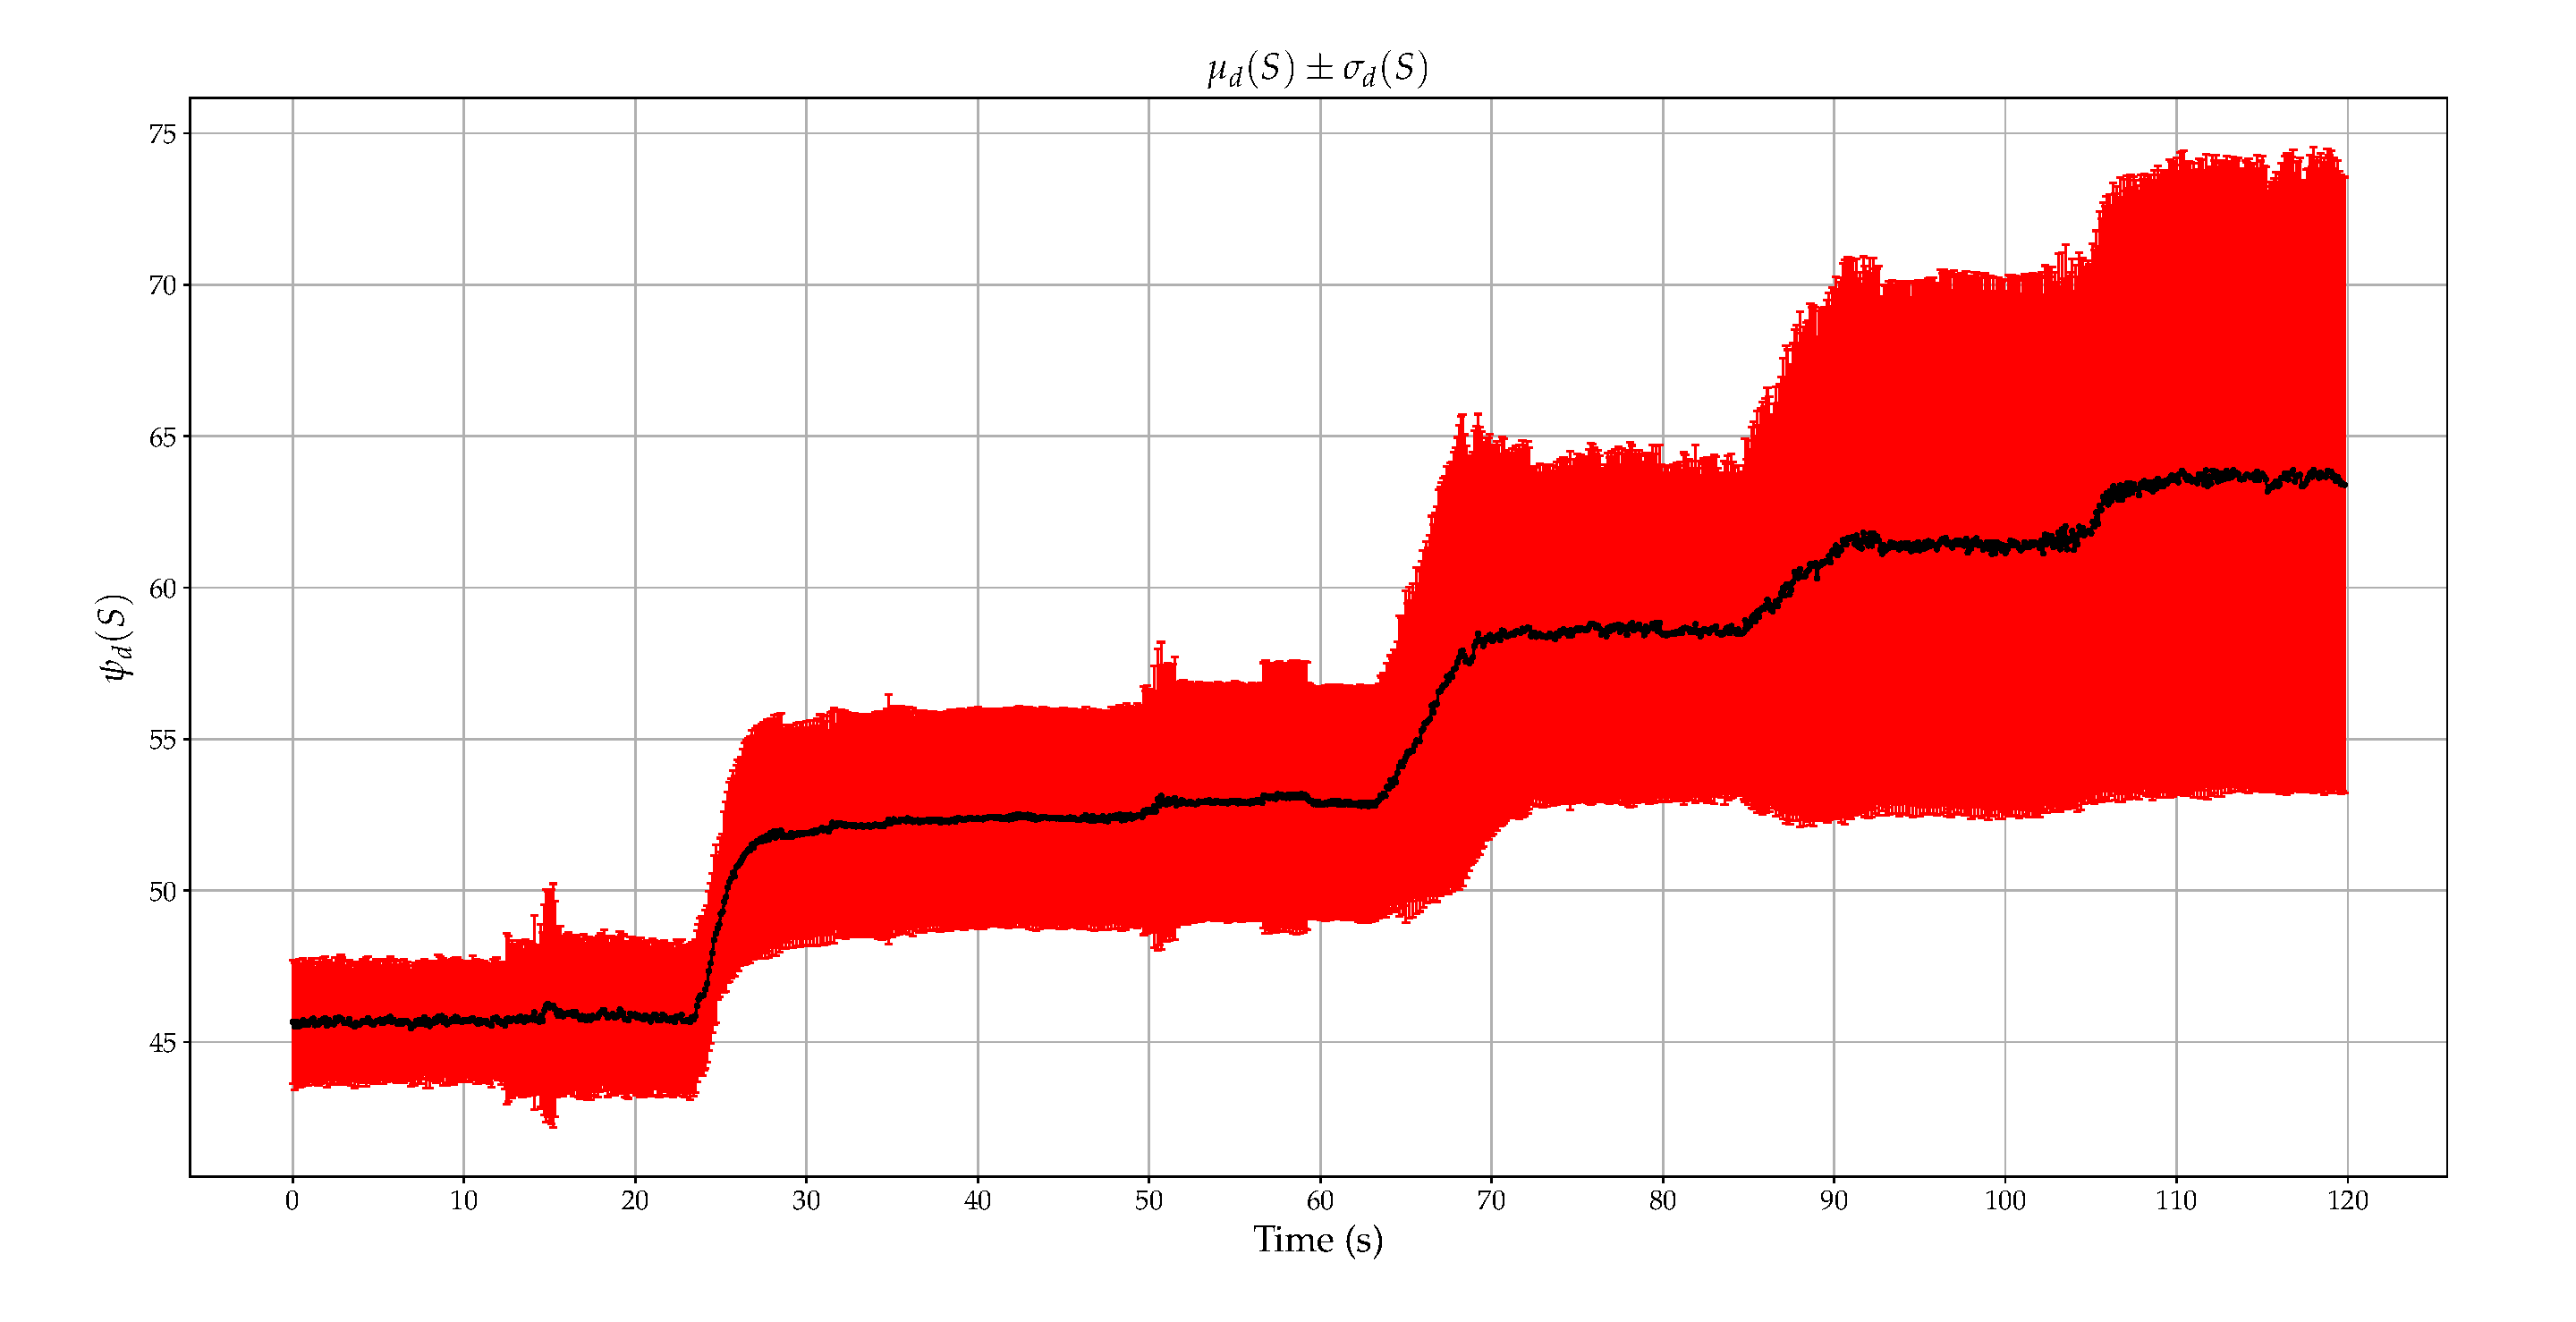
\includegraphics[width=12cm]{figures/FIELDFILL-DIST}
% \end{center}
% \caption{Distance metric 0-120 seconds\label{emerge:FIELDFILL-DIST}}
% \end{figure}

\section{Conclusion\label{metric:MagnitudeDistanceComparison}}
%% The two metrics (distance and \emph{cohesion/repulsion}) both measure the structure of a swarm in terms of the distribution of the agents and deviations from a mean. The \emph{cohesion/repulsion} metric also allows the state of the swarm to be identified.
%% 
%% The distance metric is based upon the physical \emph{distribution} of the agents and the cohesion/repulsion metric is based upon the logical \emph{interaction} of the agents.
The distance-based metric measures swarm structure in terms of position of agents.

The distance-based metric provides an analysis of the distribution of the agents at a point in time and allows the agitation of the swarm to be assessed. It does not take into account the possible distribution of agents that the field effects \emph{could} produce.

\Figure[t!](topskip=0pt, botskip=0pt, midskip=0pt)[width=6cm]{figures/FieldEffects2}
{Heterogeneous field effects.\label{additional:fieldsWork}}

The \emph{cohesion/repulsion} metric provides an indication of a swarm's potential movement. This is independent of the physical distribution of the agents within the swarm. The lack of dependence on the physical distribution allows the metric to be used in heterogeneous field effect swarms~(Fig.~\ref{additional:fieldsWork}) where the physical distribution of agents may vary due to the varied field effect ranges. 

In a homogeneous field effect swarm the two metrics together provide a deeper evaluation of a swarm's structure and `potential'. Consider the following: the repulsion field is increased but the internal distances do not change; as a result the \emph{cohesion/repulsion metric} rises: This indicates `something' is confining the swarm's distribution as discussed in Section \ref{metric:ApplicationFloodFilling}. This analysis could be used in identifying effective swarm distribution for the coverage of a sensor array as discussed by Ramaithitima et al.~\cite{RWBK:15}

%% \begin{figure}[H]
%% \begin{center}
%% \includegraphics[width=6cm]{figures/FieldEffects2}
%% \end{center}
%% \caption{Complex swarm interactions\label{additional:fieldsWork}}
%% \end{figure}

\section{Future work\label{metric:Future}}
The metric can be applied to the analysis of the effects of coordination algorithms upon a swarm's structure. An application to floodfilling has just been discussed. The metric can also be applied to identifying the effects a `healing' algorithm may have upon a swarm's structure. By this we mean an algorithm which removes `voids' in a swarm.

The detection of a swarm's perimeter \cite{MD:09, MJ:08, ZAPS:07, JG:13} identifies a subset of a swarm which can be used for coordination. The use of the perimeter detection allows a swarm to be used in many different ways~\cite{ZFG:13, AKK:08, APZDAMC:09, AZDPS:11}. 

A possible adaptation to this area of research is to use the swarm perimeter detection to identify a subset of agents then reduce the field effects (repulsion and cohesion) of those agents to increase the agent density at the perimeter, this is similar to having heterogeneous swarm structures as shown in Fig.~\ref{additional:fieldsWork}. Increasing the density would allow increased coverage of any sensor arrays that the swarm was using at the swarm edge. 

The issue with introducing heterogeneous field effects is that the existing distance-based metric would not allow the swarm's structure to be analysed correctly. We believe that cohesion/repulsion metric discussed in this paper will still identify the swarm's structure when the swarm is hetrogenious. This is due to the metric being based upon inter-agent effects rather than physical distribution. 

\clearpage

\bibliographystyle{plain}
\bibliography{thesis}

\begin{IEEEbiography}[{
\includegraphics[width=1in,height=1.25in,clip,keepaspectratio]{Images/eliot}}]{Neil Eliot} has been a Senior Lecturer at Northumbria University since 1998. Prior to this Neil worked in the chemical industry and the NHS. He was awarded his Ph.D. from Northumbria in 2017, his Pg.C. in 1994, and his B.Sc. in 1989 all in Computing. His research interests are in the area of swarm theory and cybersecurity. 
\end{IEEEbiography}

\begin{IEEEbiography}[{
\includegraphics[width=1in,height=1.25in,clip,keepaspectratio]{Images/kenda}}]{David Kendall}
has been a Senior Lecturer in Computing at Northumbria University since 1989, except for a brief period as a Lecturer in Computer Science at Durham University (2001-02). Previously, he was a Research Associate at Newcastle University (1987-89), following experience as a Senior Software Engineer in industry (1983-86). He has an M.A. degree in Literae Humaniores from Oxford University, where he studied at New College. He received M.Sc. and Ph.D. degrees in Computing Science from Newcastle University. His research interests are in the area of formal modelling and analysis of embedded systems. 
\end{IEEEbiography}

\begin{IEEEbiography}[{
\includegraphics[width=1in,height=1.25in,clip,keepaspectratio]{Images/brock}}]{Michael Brockway}
has been a Senior Lecturer at Northumbria University for 17 years. His first degree is in pure and applied mathematics (1973-4), his Masters in mathematics (mathematical logic, category theory, 1975), and he has a PhD in computer science (formal methods for distributed embedded systems, 2010) from Northumbria University. Before that Michael worked in teaching and the computing industry.
\end{IEEEbiography}

\EOD

\end{document}
